As mentioned previously, it's computationally expensive to compute the full Fisher Information. A single matrix for the smallest network from the previous section would already be over 50GB in size. Therefore, to be able to compute and visualize the trace of the NTK, the Fisher Information and the curvature $R$, this section covers the training of one of the simplest networks possible. It's simplicity allows us to compute the observables for a whole grid of parameters instead of just the path of parameters during in training.

\subsection{The network}
The network used for the experiment in \cref{sec:ResultsOf2ParameterNetwork} consists of a single neuron with two inputs, two weights but no bias. It uses a sigmoid function \cite{ActivationFunctionOverview} as its activation function. This means that we can express the output of the network by 
\begin{equation}\label{eq:Results2Sigmoid}
	f_\theta(x,y) = \frac{1}{1+ \exp (-5(\theta_1 x + \theta_2 y))},
\end{equation}
with inputs $x$ and $y$. The factor $5$ was added to make the sigmoid function steeper. The network output, which is a number between $0$ and $1$, represents prediction whether the input data belongs to the class with target $0$ or the class with target $1$.\\
The loss functions considered are the same as in \cref{sec:Results1}.

\subsection{The dataset}
The dataset used in \cref{sec:ResultsOf2ParameterNetwork} is depicted in \cref{fig:DB dataset}. We created the input data by generating a set of randomly distributed $(x,y)$ pairs within the square from $0$ to $1$. The input pair is sorted into the class of target $1$ if the $y$ coordinate is bigger than the $x$ coordinate, and in the 
\begin{figure}
	\centering
	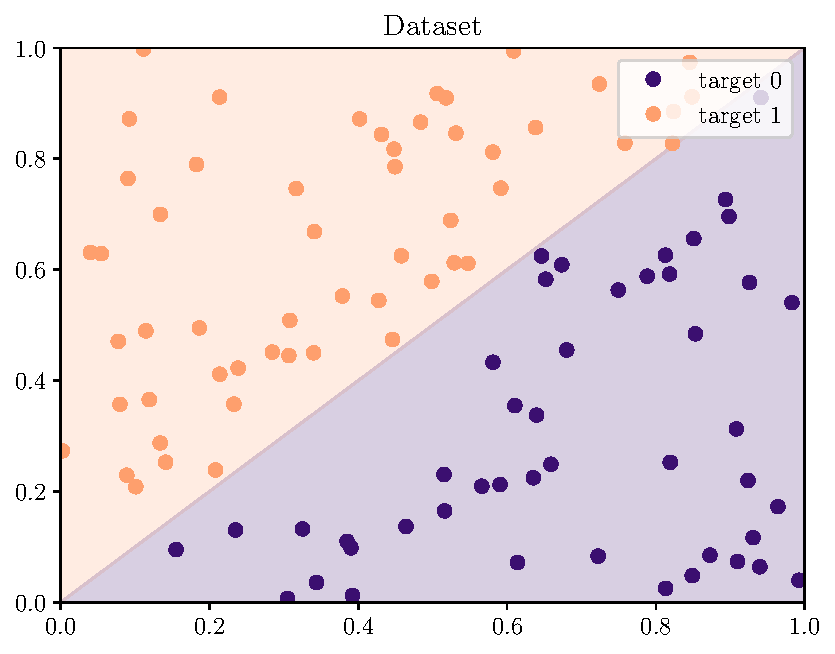
\includegraphics{Experiment2/plots/Dataset.pdf}
	\caption{The decision boundary dataset used in the creation of the data from \cref{sec:ResultsOf2ParameterNetwork}.}
	\label{fig:DB dataset}
\end{figure}

\subsection{Results}\label{sec:ResultsOf2ParameterNetwork}
To start of this analysis, let's inspect the loss surfaces of the network depicted in \cref{fig:Results2LossSurfaces}.
\begin{figure}
	\centering
	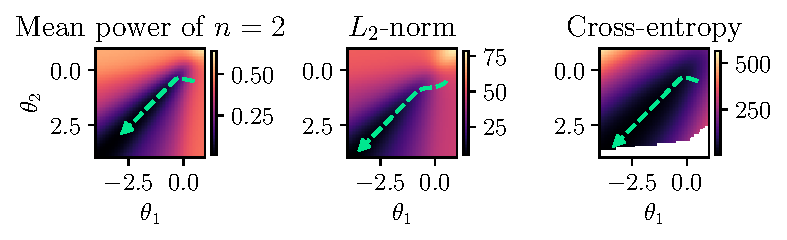
\includegraphics{Experiment2/plots/LossSurfaces.pdf}
	\caption{Loss surfaces for the three considered loss functions. The path of the parameters during gradient descent with initialization at $\theta = \{0.5, 0.5\}$ is depicted as a dotted line.}
	\label{fig:Results2LossSurfaces}
\end{figure}
In every case, the loss surface has a valley along the line of $-\theta_1 = \theta_2$, leading down towards increasing values of  $\theta_2$. This makes sense, considering that the network output from \cref{eq:Results2Sigmoid} is larger than $0.5$ for $\theta_1x + \theta_2y < 0$ and smaller than $0$ otherwise. Since we want the network outputs for inputs with $y>x$ to be $1$, we want the parameters to be $\theta_1 = - \theta_2$ with large absolute values. The loss functions differ in the actual shape of the valley.\\
The path of the parameters during training with Gradient Descent is depicted as a dotted line in the figure. To make the training look similar throughout different loss surfaces and different trials, we initialized the training at $\theta = \{0.5, 0.5\}$ instead of choosing random starting points. Since the actual values of the loss also vary throughout the loss surfaces, we adjusted the learning rate and number of training epochs to account for the resulting variations in the size of gradients. In all cases, the network predicted all of the datapoints correctly at the end of training.\\
For some of the surfaces depicted here and in later figures, parts of the heatmap are missing. This is due to computational failure. We didn't investigate this further, since the missing parts seem to be predictable from the visible data in most cases.\\
To visualize the network behavior at the end of training, the output as a function of input values for the final parameters of the Cross-entropy training is depicted in \cref{fig:Results2NetworkOutput}.
\begin{figure}
	\centering
	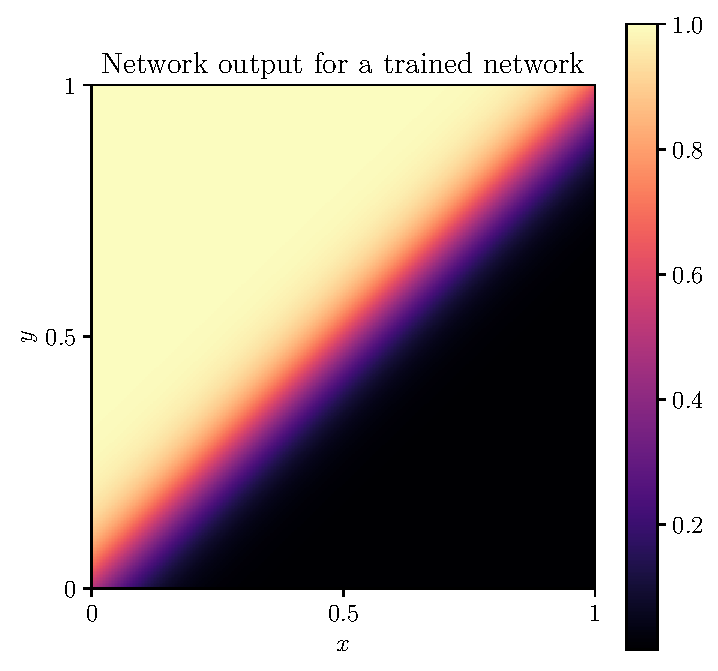
\includegraphics{Experiment2/plots/Network_output.pdf}
	\caption{Network output at the final parameters of training on the Cross-entropy loss.}
	\label{fig:Results2NetworkOutput}	
\end{figure}
Now let's look at the surfaces for the Fisher Information $I$, its trace $\mathrm{tr}(I)$, the trace of the NTK $\mathrm{tr}(\Lambda)$ and the scalar curvature $R$. The results for Mean power loss of order $n=2$ are depicted in \cref{fig:Results2MeanPowerLoss}, the results for $L_2$-norm loss are depicted in \cref{fig:Results2LPNormLoss} and the results for Cross-entropy loss are depicted in \cref{fig:Results2CrossEntropyLoss}. The path of the parameters is depicted in every heatmap, similar to \cref{fig:Results2LossSurfaces}.\\
\begin{figure}
	\centering
	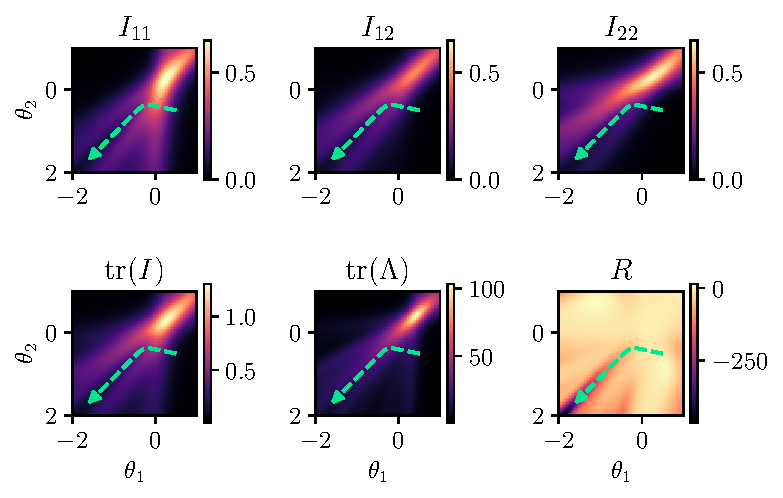
\includegraphics{Experiment2/plots/MeanPowerLoss2_tracecomparison.pdf}
	\caption{Surfaces of all components of the Fisher Information $I$, its trace $\mathrm{tr}(I)$, the trace of the NTK $\mathrm{tr}(\Lambda)$ and the scalar curvature $R$ for \emph{Mean power loss of order $n=2$}.}
	\label{fig:Results2MeanPowerLoss}
\end{figure}

\begin{figure}
	\centering
	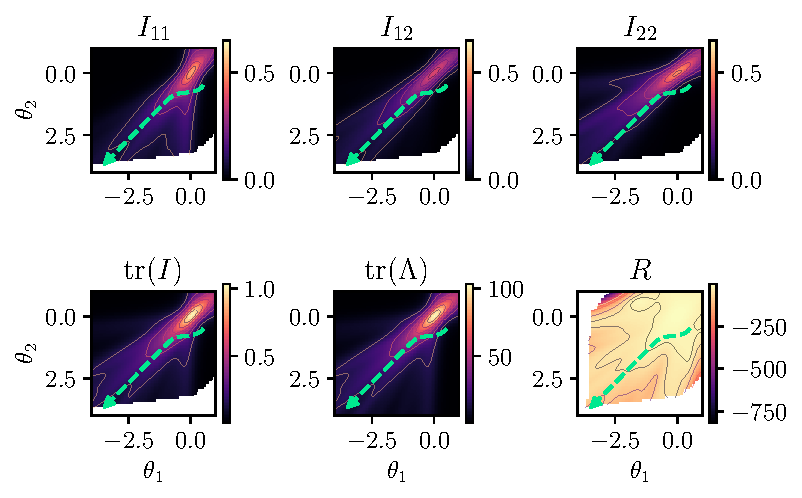
\includegraphics{Experiment2/plots/LPNormLoss2_tracecomparison.pdf}
	\caption{Surfaces of all components of the Fisher Information $I$, its trace $\mathrm{tr}(I)$, the trace of the NTK $\mathrm{tr}(\Lambda)$ and the scalar curvature $R$ for \emph{$L_2$-norm loss}.}
	\label{fig:Results2LPNormLoss}
\end{figure}

\begin{figure}
	\centering
	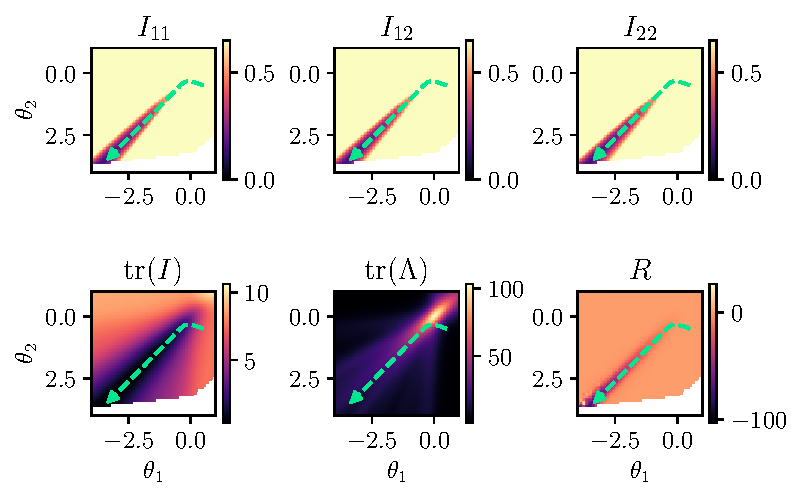
\includegraphics{Experiment2/plots/CrossEntropyLoss_tracecomparison.pdf}
	\caption{Surfaces of all components of the Fisher Information $I$, its trace $\mathrm{tr}(I)$, the trace of the NTK $\mathrm{tr}(\Lambda)$ and the scalar curvature $R$ for \emph{Cross-entropy loss}.}
	\label{fig:Results2CrossEntropyLoss}
\end{figure}


In addition to those plots, we can inspect the evolution of the traces and the curvature along the path of parameters during training. The resulting curves are depicted in \cref{fig:Results2MeanPowerLossCurves} for the Mean power loss of order $n=2$, \cref{fig:Results2LPNormLossCurves} for $L_2$-norm loss and \cref{fig:Results2CrossEntropyLossCurves} for Cross-entropy loss.

\begin{figure}
	\centering
	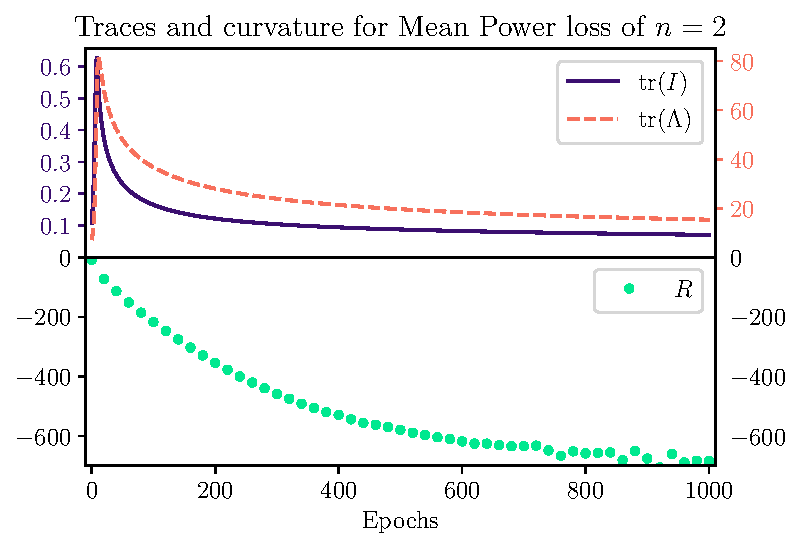
\includegraphics{Experiment2/plots/MeanPowerLoss2_Curves.pdf}
	\caption{Evolution of the Fisher Trace, the NTK Trace and the scalar curvature during training with GD and \emph{Mean power loss of order $n=2$}.}
	\label{fig:Results2MeanPowerLossCurves}
\end{figure}

\begin{figure}
	\centering
	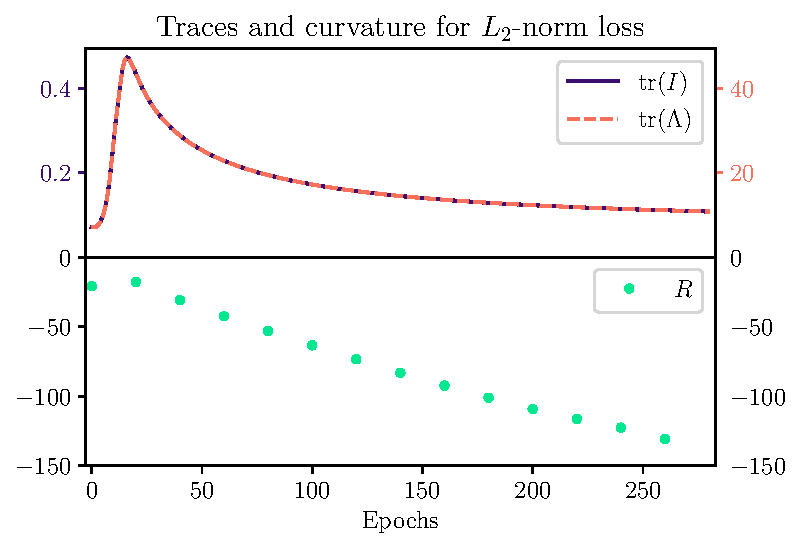
\includegraphics{Experiment2/plots/LPNormLoss2_Curves.pdf}
	\caption{Evolution of the Fisher Trace, the NTK Trace and the scalar curvature during training with GD and \emph{$L_2$-norm loss}.}
	\label{fig:Results2LPNormLossCurves}
\end{figure}

\begin{figure}
	\centering
	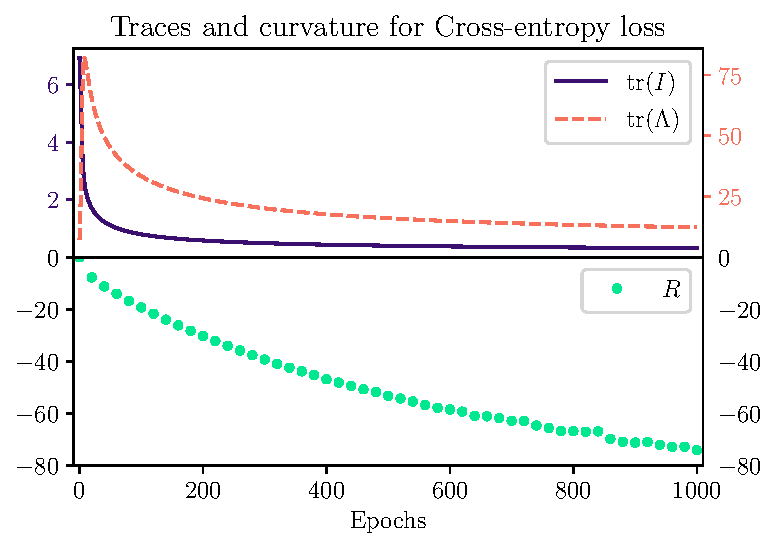
\includegraphics{Experiment2/plots/CrossEntropyLoss_Curves.pdf}
	\caption{Evolution of the Fisher Trace, the NTK Trace and the scalar curvature during training with GD and \emph{Cross-entropy loss}.}
	\label{fig:Results2CrossEntropyLossCurves}
\end{figure}

Although we can't fully explain the shape of these surfaces, we can note a few key details.\\
First, similar to the results of \cref{sec:Results1}, the Fisher Trace and the NTK trace behave similarly for the $L_2$-norm loss. In fact, for this experiment they are indistinguishable to each other apart from a constant factor. This means that the loss derivatives from \cref{eq:FisherNTKRelation} don't depend on the input index $i$. For the other loss functions, the traces also behave more similar than the traces in the MNIST experiment. We'd also expect this behavior, since the input values, representing points on a 1 by 1 square in $\mathrm{R}^2$ are less diverse than the $R^{784}$ pictures of handwritten digits. It's a reasonable assumption that this also makes the loss derivatives with respect to the output of those input points less diverse. Since the network used here only outputs one value, we also lose an extra summation in \cref{eq:FisherNTKRelation}. Those factors in combination lead to the Fisher Trace being closer related to the NTK Trace.\\
For this experiment we also measured the scalar curvature $R$. We calculated it from the Fisher Information using the equations presented in \cref{sec:Curvature}. The resulting algorithm was tested against multiple reference matrices with the help of analytical results from the EinsteinPy package \cite{EinsteinPyPackage}. Here we can note that the curvature seems to descend roughly linearly in the first parts of training, although the graph for the Cross-entropy loss hints at it possibly converging for further training. It's also important to note that its always negative and the path of the parameters descends into a valley of high negative curvature that is more narrow than the valley of the loss function. For the $L_2$-norm loss the valley isn't visible in the surface heatmap, but it gets clear that the curvature still descends in \cref{fig:Results2LPNormLossCurves}. What exactly large negative curvature means for the manifold of neural network training, and if the networks always tend to negative values is not fully understood yet.